\begin{figure}[H]

    \centering
    \tikzset{every picture/.style={line width=0.75pt}} %set default line width to 0.75pt

    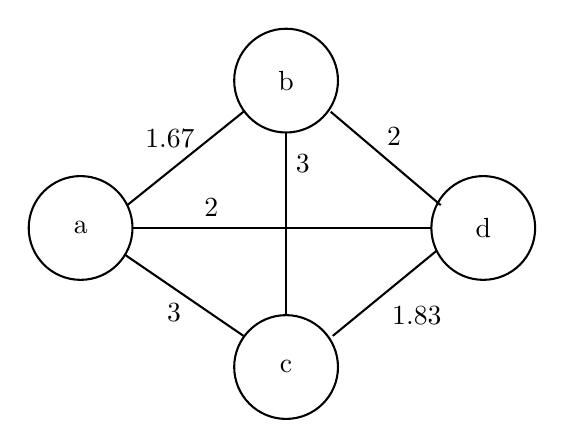
\begin{tikzpicture}[x=0.75pt,y=0.75pt,yscale=-1,xscale=1]
        %uncomment if require: \path (0,300); %set diagram left start at 0, and has height of 300

        %Shape: Circle [id:dp14719016101017623]
        \draw   (111,126) .. controls (111,112.19) and (122.19,101) .. (136,101) .. controls (149.81,101) and (161,112.19) .. (161,126) .. controls (161,139.81) and (149.81,151) .. (136,151) .. controls (122.19,151) and (111,139.81) .. (111,126) -- cycle ;
        %Shape: Circle [id:dp637969227645387]
        \draw   (210,55) .. controls (210,41.19) and (221.19,30) .. (235,30) .. controls (248.81,30) and (260,41.19) .. (260,55) .. controls (260,68.81) and (248.81,80) .. (235,80) .. controls (221.19,80) and (210,68.81) .. (210,55) -- cycle ;
        %Shape: Circle [id:dp16996306115691606]
        \draw   (210,193) .. controls (210,179.19) and (221.19,168) .. (235,168) .. controls (248.81,168) and (260,179.19) .. (260,193) .. controls (260,206.81) and (248.81,218) .. (235,218) .. controls (221.19,218) and (210,206.81) .. (210,193) -- cycle ;
        %Shape: Circle [id:dp4723269788902422]
        \draw   (305,126) .. controls (305,112.19) and (316.19,101) .. (330,101) .. controls (343.81,101) and (355,112.19) .. (355,126) .. controls (355,139.81) and (343.81,151) .. (330,151) .. controls (316.19,151) and (305,139.81) .. (305,126) -- cycle ;
        %Straight Lines [id:da43115389914855107]
        \draw    (158.5,115) -- (214.5,70) ;


        %Straight Lines [id:da3262134359528708]
        \draw    (257.5,178) -- (307.5,137) ;


        %Straight Lines [id:da6644861489456326]
        \draw    (235,168) -- (235,80) ;


        %Straight Lines [id:da44726258546505226]
        \draw    (157.5,139) -- (214.5,178) ;


        %Straight Lines [id:da17516578825824003]
        \draw    (309.5,115) -- (256.5,70) ;


        %Straight Lines [id:da25861424028019475]
        \draw    (161,126) -- (305,126) ;



        % Text Node
        \draw (136,126) node  [align=left] {a};
        % Text Node
        \draw (235,55) node  [align=left] {b};
        % Text Node
        \draw (235,193) node  [align=left] {c};
        % Text Node
        \draw (330,126) node  [align=left] {d};
        % Text Node
        \draw (179,83) node  [align=left] {1.67};
        % Text Node
        \draw (181,167) node  [align=left] {3};
        % Text Node
        \draw (199,116) node  [align=left] {2};
        % Text Node
        \draw (243,95) node  [align=left] {3};
        % Text Node
        \draw (287,82) node  [align=left] {2};
        % Text Node
        \draw (298,168) node  [align=left] {1.83};


    \end{tikzpicture}

    \caption{Example cost-graph}\label{fig:cost_graph}
\end{figure}